\section{Michal Fidelus}
\label{sec:mfidelus}

Gekon (patrz Figure~\ref{fig:geck}).

\begin{figure}[htbp]
    \centering
    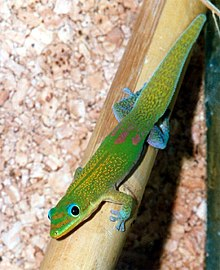
\includegraphics[width=0.8\textwidth]{pictures/geck.jpg}
    \caption{Gekony są super}
    \label{fig:geck}
\end{figure}



\begin{table}[htbp]
\centering
\begin{tabular}{||c c c ||} 
 \hline
 Col1 & Col2 & Col2 \\ [1ex] 
 \hline\hline
 137 & 371 & 713   \\
 \hline
 713 & 137 & 371  \\
 \hline
 371 & 713 & 137  \\
 \hline
\end{tabular}
\label{tab:random_numbers}
\caption{tablee.}
\end{table}


Matematyka: 
\[−x+2⋅y+z=−1\]

Równanie matematyczne:
$12x - 9x = 10 - 7$